% !TEX TS-program = pdflatex
% !TEX encoding = UTF-8 Unicode

% This is a simple template for a LaTeX document using the "article" class.
% See "book", "report", "letter" for other types of document.

\documentclass[11pt]{article} % use larger type; default would be 10pt

\usepackage[utf8]{inputenc} % set input encoding (not needed with XeLaTeX)
\usepackage{gensymb}
\usepackage[hidelinks]{hyperref}
%%% Examples of Article customizations
% These packages are optional, depending whether you want the features they provide.
% See the LaTeX Companion or other references for full information.

%%% PAGE DIMENSIONS
\usepackage{geometry} % to change the page dimensions
\geometry{a4paper} % or letterpaper (US) or a5paper or....
% \geometry{margin=2in} % for example, change the margins to 2 inches all round
% \geometry{landscape} % set up the page for landscape
%   read geometry.pdf for detailed page layout information

\usepackage{graphicx} % support the \includegraphics command and options
\usepackage{wrapfig}
 \usepackage[font=footnotesize,labelfont=bf]{caption} %changes caption size
% \usepackage[parfill]{parskip} % Activate to begin paragraphs with an empty line rather than an indent

%%% PACKAGES
\usepackage{booktabs} % for much better looking tables
\usepackage{array} % for better arrays (eg matrices) in maths
\usepackage{paralist} % very flexible & customisable lists (eg. enumerate/itemize, etc.)
\usepackage{verbatim} % adds environment for commenting out blocks of text & for better verbatim
\usepackage{subfig} % make it possible to include more than one captioned figure/table in a single float
% These packages are all incorporated in the memoir class to one degree or another...

%%% HEADERS & FOOTERS
\usepackage{fancyhdr} % This should be set AFTER setting up the page geometry
\pagestyle{fancy} % options: empty , plain , fancy
\renewcommand{\headrulewidth}{0pt} % customise the layout...
\lhead{}\chead{}\rhead{}
\lfoot{}\cfoot{\thepage}\rfoot{}

%%% SECTION TITLE APPEARANCE
\usepackage{sectsty}
\allsectionsfont{\sffamily\mdseries\upshape} % (See the fntguide.pdf for font help)
% (This matches ConTeXt defaults)

%%% ToC (table of contents) APPEARANCE
\usepackage[nottoc,notlof,notlot]{tocbibind} % Put the bibliography in the ToC
\usepackage[titles,subfigure]{tocloft} % Alter the style of the Table of Contents
\renewcommand{\cftsecfont}{\rmfamily\mdseries\upshape}
\renewcommand{\cftsecpagefont}{\rmfamily\mdseries\upshape} % No bold!


%%% END Article customizations

%%% The "real" document content comes below...


\date{} % Activate to display a given date or no date (if empty),
         % otherwise the current date is printed 
\title{Glucocorticoid-Induced Metabolic Disturbances are Exacerbated in
Obesity}

\author{Innocence Harvey\footnote{Department of Nutritional Sciences, University of Michigan School of Public Health, Ann Arbor, MI} \footnote{Department of Physiology, University of Tennessee Health Science Center, Memphis, TN}, Erin J. Stephenson \textsuperscript{$\dagger$}\footnote{Department of Pediatrics, University of Tennessee Health Science Center, Memphis, TN} , JeAnna R. Redd\textsuperscript{$\ast$,$\dagger$} ,\\ Quynh T. Tran\footnote{Department of Preventive Medicine, University of Tennessee Health Science Center, Memphis, TN},
Irit Hochberg\footnote{ Institute of Endocrinology, Diabetes and Metabolism, Rambam Health Care Campus, Haifa, Israel}, Nathan Qi\footnote{Metabolism, Endocrinology \& Diabetes, University of Michigan Medical School, Ann Arbor, MI} and Dave Bridges\textsuperscript{$\ast$,$\dagger$,$\ddagger$,} \footnote{Please address any correspondance to \href{mailto:davebrid@umich.edu}{davebrid@umich.edu}}}

\begin{document}
\maketitle

\abstract{Objective: To determine the effects of glucocorticoid-induced metabolic dysfunction in the presence of diet-induced obesity.
Methods: C57BL/6J adult male lean and diet-induced obese mice were given dexamethasone for different durations and levels of hepatic steatosis, insulin resistance and lipolysis were determined.
Results: Obese mice given dexamethasone had significant, synergistic effects on insulin resistance and markers of lipolysis, as well as hepatic steatosis.  This was associated with synergistic transactivation of the lipolytic enzyme ATGL.
Conclusions: The combination of chronically elevated glucocorticoids and obesity leads to exacerbations in metabolic dysfunction. Our findings suggest lipolysis may be a key player in glucocorticoid-induced insulin resistance and fatty liver in individuals with obesity.} 

\section*{Introduction} 

Cushing's syndrome manifests in response to chronically elevated levels
of glucocorticoids and is often associated with changes in adipose mass
and distribution, non-alcoholic fatty liver disease (NAFLD) and impaired
glucose tolerance (Paredes \& Ribeiro 2014). While Cushing's disease is
rare, it is estimated that at any given time 1-3\% of the US, UK and
Danish populations are prescribed exogenous corticosteroids, which may
increase their risk for developing the metabolic complications (Hsiao
\emph{et al.} 2010; Fardet \emph{et al.} 2011; Overman \emph{et al.}
2013; Laugesen \emph{et al.} 2017).

Similarly, obesity is accompanied by a multitude of metabolic
disturbances, such as insulin resistance and NAFLD and is a worldwide
epidemic (The GBD 2015 Obesity Collaborators 2017). Comparing the high
rates of medically prescribed corticosteroids with the prevalence of
overweight and obesity in developed countries, the combination of
obesity and glucocorticoid excess may be present in many individuals.
Given the similar co-morbidities associated with obesity and chronically
elevated glucocorticoids, we hypothesized that the combinations of these
two conditions would lead to worse metabolic outcomes than either of
them alone. This is supported by studies in rats showing that
corticosterone and high-fat diets combine to cause worsened insulin
resistance and non-alcoholic fatty liver disease (Shpilberg \emph{et
al.} 2012; Beaudry \emph{et al.} 2013).

There is an array of physiological changes that occur as a result of
elevated glucocorticoids including decreased lean mass (Dardevet
\emph{et al.} 1995; Schakman \emph{et al.} 2013; Hochberg \emph{et al.}
2015), increased fat mass (Abad \emph{et al.} 2001; Geer \emph{et al.}
2011; Hochberg \emph{et al.} 2015), NAFLD (Shpilberg \emph{et al.} 2012)
and increased lipolysis (Djurhuus \emph{et al.} 2002, 2004; Kršek
\emph{et al.} 2006), all of which have been associated with decreased
insulin sensitivity (Rebrin \emph{et al.} 1996; Zhang \emph{et al.}
2015; Dirks \emph{et al.} 2016). Recent tissue-specific knockouts of
glucocorticoid signaling mediators have implicated adipose tissue as a
central node linking glucocorticoid action and lipolysis to systemic
insulin resistance and NAFLD (Morgan \emph{et al.} 2014; Wang \emph{et
al.} 2014; Mueller \emph{et al.} 2017; Shen \emph{et al.} 2017). Here we
present the finding that chronically elevated glucocorticoids in the
presence of diet-induced obesity have synergistic effects on lipolysis,
insulin resistance and fatty liver disease. Obese glucocorticoid-treated
mice have reduced fat mass compared to all other groups, yet have
hyperglycemia and severe insulin resistance. Therefore, we speculate
that lipolysis drives insulin resistance in obese animals.

\section*{Methods}

\textbf{Animal Procedures:} C57BL/6J adult male mice were purchased from
the Jackson Laboratory at nine weeks of age (stock \#000664). All
animals were on a light dark cycle of 12/12 h and housed at 22\degree C.
Following a week of acclimation, mice were placed on diets or treated
with dexamethasone as described in the figure legends. Mice were treated
with vehicle (water) or approximately 1mg/kg/d of water-soluble
dexamethasone (Sigma-Aldrich; catalog \#2915) dissolved in their
drinking water for 12 weeks, as described previously (Hochberg \emph{et
al.} 2015). Additional cohorts of mice used in these experiments either
remained on a standard diet (normal chow diet; NCD; 5L0D LabDiet; 13\%
fat; 57\% carbohydrate; 30\% protein) or were provided a high fat diet
(45\% fat from lard; 35\% carbohydrate mix of starch, maltodextrin and
sucrose; 20\% protein from casein; cat\# D12451) for either 8 or 12
weeks followed by dexamethasone treatment. Mice were group housed with
four mice per cage and food consumption was measured weekly by weight
reductions per cage and calculated to reflect estimated intake of each
mouse per day in a given cage. Mice remained on their respective diets
for the duration of the study. All mice were provided with access to
food and water~\emph{ad libitum}~throughout the study, unless otherwise
noted. For the longer, six-week dexamethasone treatments, 16 HFD-fed,
dexamethasone-treated mice appeared ill and were euthanized and thus
removed from all analyses once symptoms were noticed. Symptoms included
lethargy, weight loss and evidence of pancreatitis in some of the mice.
Animal body weight and composition was determined weekly using a digital
scale and EchoMRI 2100, respectively. We performed a CLAMS experiment
(data not shown) with the 12-week diet study prior to dexamethasone
treatment where mice were singly housed for approximately one week,
which led to fluctuations in body weight over the first week. Body
weight quickly stabilized following removal from the CLAMS in both
groups. At the end of treatment, mice were fasted for 16 h,
dexamethasone water was not removed during this time, and euthanized by
cervical dislocation after isoflurane anesthesia at ZT3. Immediately
following euthanasia, mice were dissected and the right inguinal white
adipose tissue (iWAT) and epididymal white adipose tissue (eWAT) depots
were carefully removed and weighed. Adipose tissues, along with a
section of the left lateral lobe of the liver were snap frozen in liquid
nitrogen for later analysis. Small pieces of tissues were fixed in 10\%
phosphate-buffered formalin for histology. Animal procedures were
approved by the University of Tennessee Health Science Center and
University of Michigan Institutional Animal Care and Use Committees.

\textbf{Insulin Tolerance Tests and Hyperinsulinemic Euglycemic Clamp
Experiments:} Insulin responsiveness was assessed via an insulin
tolerance test (ITT). Following a six hour fast, mice were given an
intraperitoneal (IP) injection of insulin (Humulin R, Lilly,) as
described in figure legends. Blood was collected from the tail and
glucose was determined using a One Touch Ultra Glucometer (Lifescan ).
For the hyperinsulinemic euglycemic clamp experiments, C57BL/6J adult
(70d) male mice were fed HFD for eight weeks and treated with
dexamethasone in their drinking water for three weeks or regular
drinking water. Animals were anesthetized with an IP injection of sodium
pentobarbital (50−60 mg/kg). Indwelling catheters were inserted into the
right jugular vein and the right carotid artery, respectively.~ The free
ends of catheters were tunneled subcutaneously and exteriorized at the
back of the neck via a stainless-steel tubing connector (coated with
medical silicone) that was fixed subcutaneously upon closure of the
incision. Animals with healthy appearance, normal activity, and weight
regain to or above 90\% of their pre-surgery levels were used for the
study. Experiments were carried out in conscious and unrestrained
animals using techniques described previously (Halseth \emph{et al.}
1999; Ayala \emph{et al.} 2006; McGuinness \emph{et al.} 2009). Briefly,
the primed (1.0~$\mu$Ci)-continuous infusion (0.05~$\mu$Ci/min and increased to
0.1 $\mu$Ci/min at t = 0) of {[}3-\textsuperscript{3}H{]} glucose (50 $\mu$Ci/ml
in saline) was started at t = -120min. After a five-hour fast, the
insulin clamp was initiated at t = 0, with a prime-continuous infusion
(40 mU/kg bolus, followed by 8.0 mU/kg/min) of human insulin (Novo
Nordisk). Euglycemia (120\textasciitilde{}130 mg/dL) was maintained
during the clamp by measuring blood glucose every 10 min and infusing
50\% glucose at variable rates, accordingly.~ Blood samples were
collected from the right carotid artery at t = 80, 90, 100, and 120 min
for determination of glucose specific activity.~ Blood insulin
concentrations were determined from samples taken at t = -10 and 120
min. A bolus injection of {[}1-\textsuperscript{14}C{]}-2-deoxyglucose
({[}\textsuperscript{14}C{]}2DG; PerkinElmer) (10 $\mu$Ci) was given at t =
120 min. Blood samples were taken at 2, 5, 10, 15, and 25 min after the
injection for determination of plasma {[}\textsuperscript{14}C{]}2DG
radioactivity. At the end of the experiment, animals were anesthetized
with an intravenous injection of sodium pentobarbital and tissues were
collected and immediately frozen in liquid nitrogen for later analysis
of tissue {[}1-\textsuperscript{14}C{]}-2-deoxyglucose phosphate
({[}\textsuperscript{14}C{]}2DGP) radioactivity. Blood glucose was
measured using an Accu-Chek glucometer (Roche, Germany). Plasma insulin
was measured using the Linco rat/mouse insulin ELISA kits.~ For
determination of plasma radioactivity of
{[}3-\textsuperscript{3}H{]}glucose and
{[}1-\textsuperscript{14}C{]}2DG, plasma samples were deproteinized with
ZnSO\textsubscript{4}~and Ba(OH)\textsubscript{2}~and counted using a
Liquid Scintillation Counter (Beckman Coulter LS6500 Multi-purpose
Scintillation Counter). Glucose turnover rate, hepatic glucose
production and tissue glucose uptake were calculated as described
elsewhere (Kraegen \emph{et al.} 1985; Halseth \emph{et al.} 1999; Ayala
\emph{et al.} 2006).

\textbf{Serum Glycerol and Fatty Acid Determination:} Following 12 weeks
of dexamethasone treatment, 22-week-old \emph{ad libitum} chow fed
C57BL/6J male mice were anesthetized with isoflurane and blood was
collected into heparin-coated capillary tubes via retro orbital bleed
both prior to and 15 minutes following intraperitoneal injection of
10mg/kg isoproterenol (Sigma-Aldrich; catalog \#I6504-1G) in Dulbecco's
phosphate-buffered saline (Thermo Fisher; catalog \#BW17512F1). Serum
from these mice, as well as from a cohort of 28-week old mice on either
HFD or chow, six-weeks post-dexamethasone treatment was collected
following an overnight fast. Glycerol was assessed via Serum
Triglyceride Determination Kit (Sigma-Aldrich; catalog \#TR0100-1KT) and
fatty acids were quantified using the HR Series NEFA-HR(2) kit (Wako
Diagnostics; catalog \#276-76491), in accordance with manufacturer's
guidelines.

\textbf{Cell culture:} 3T3-L1 fibroblasts (pre-adipocytes; ATCC;
authenticated via STRS analysis) were cultured in 10\% newborn calf
serum, Dulbecco's Modification of Eagle's Medium (DMEM; 4.5 g/L
D-glucose; Fisher Scientific; catalog \#11965118) with penicillin,
streptomycin and glutamine (PSG) until confluence. Cells were switched
to a differentiation cocktail at two days post confluence (250nM
dexamethasone, 500$\mu$M 3-isobutyl-1-methylxanthine and 1$\mu$g/mL insulin in
10\% fetal bovine serum, in 4.5g/L glucose DMEM with PSG) for four days
(Chiang S-H, Chang L 2002). Media was replaced with differentiation
medium containing only insulin for an additional three days. For the
following three days, cells remained in media with no additional
treatment. Cells used for these experiments were not cultured beyond 22
passages. To assess markers of lipolysis, cells remained in media and
were treated with ethanol (vehicle) or 250nM dexamethasone for five days
before lysing.

\textbf{Assessment of Triglyceride Content in Cells and Tissue:} 3T3-L1
cells were grown and treated as described above. At the end of the
treatment period, cells were lysed in homogenization buffer (50 mM Tris
pH 8, 5 mM EDTA, 30 mM Mannitol, protease inhibitor) and subjected to
three freeze thaw cycles with liquid nitrogen, thawed at room
temperature. Frozen liver tissue was homogenized using a TissueLyser II
(Qiagen). Lipids were extracted using KOH and a chloroform to methanol
(2:1) extraction. Triglyceride content was assessed using the Serum
Triglyceride Determination Kit and absorbance was detected as described
in (Lu \emph{et al.} 2014).

\textbf{Histology:} Tissues were fixed in 10\% phosphate-buffered
formalin for 24 hours and then stored in 70\% ethanol until further
processing. Tissues were dehydrated, embedded in paraffin and sent to
the University of Michigan Comprehensive Cancer Center Tissue Core where
they were processed and stained with hematoxylin and eosin (H\&E) to
assess cell morphology. Slides were imaged using the 10x objective of an
Olympus iX18 inverted microscope and cellSense software.

\textbf{mRNA Extraction and Analysis:} Cells and tissues were lysed in
TRIzol using the TissueLyser II, as decribed above, and RNA was
extracted using a PureLink RNA kit (Life Technologies; catalog
\#12183025). cDNA was synthesized from 0.5-1$\mu$g of RNA using the High
Capacity Reverse Transcription Kit (Life Technologies; catalog
\#4368813). Primers, cDNA and Power SYBR Green PCR Master Mix (Life
Technologies; catalog \#4368708) were combined in accordance with the
manufacturer's guidelines and quantitative real-time PCR (qPCR) was
performed as previously described (Lu \emph{et al.} 2014) using the
QuantStudio 5 (Thermo Fisher Scientific). mRNA expression level was
normalized to \emph{Actb} and analyzed using the $\Delta$$\Delta$ Ct method after
evaluation of several reference genes. qPCR primer sequences are listed
in Table 1.


\begin{table}[]
\centering
\caption{Primers used for RT-qPCR analyses.}
\label{my-label}
\begin{tabular}{|l|l|l|}
\hline
\textbf{Gene}   & \textbf{Forward Sequence} & \textbf{Reverse Sequence} \\ \hline
\textit{Actb}   & ATGTGGATCAGCAAGCAGGA      & AAGGGTGTAAAACGCAGCTCA     \\ \hline
\textit{Fasn}   & GGAGGTGGTGATAGCCGGTAT     & TGGGTAATCCATAGAGCCCAG     \\ \hline
\textit{Pnpla2} & CCACTCACATCTACGGAGCC      & GATGCAGAGGACCCAGGAAC      \\ \hline
\textit{Srebf1} & AGGCCATCGACTACATCCG       & TCCATAGACACATCTGTGCCTC    \\ \hline
\end{tabular}
\end{table}


\textbf{Protein Extraction and Analysis:} Cells and tissues were lysed
in RIPA buffer (50 mM Tris, pH 7.4, 0.25\% sodium deoxycholate, 1\%
NP40, 150 mM sodium chloride, 1 mM EDTA, 100 uM sodium orthovanadate, 5
mM sodium fluoride, 10 mM sodium pyrophosphate and 1x protease
inhibitor), centrifuged at 14,000rpm for 10 minutes at 4\degree C. Lysates were
heated with loading buffer at 85-95\degree C and proteins were separated by
SDS-PAGE (Life Technologies) and transferred onto nitrocellulose
membranes overnight at room temperature. Membranes were blotted at room
temperature using anti-adipose triglyceride lipase antibodies (ATGL; 54
kDa; Cell Signaling Technologies; catalog \#30A4). Antibody complexes
were detected by anti-mouse and anti-rabbit fluorescent conjugated
antibodies (Invitrogen) and visualized using an Odyssey CLx image
scanner. Blots were quantified using Image Studio software version 5.2
(LiCOR) and normalized to Revert Total Protein Stain (LiCOR; catalog
\#926-11011).

\textbf{Statistics}: All data are presented as mean +/- standard error
of the mean. For animal studies, two-way ANOVA analyses were performed
to test for significance of diet and dexamethasone treatment, as well as
their interaction. Pairwise comparisons, normality and equal variance
were tested using Shapiro-Wilk and Levene's tests, respectively. Pending
those results, a Mann-Whitney, Welch's or Student's \emph{t}-test were
used. P-values below p=0.05 were considered significant. All statistical
tests were performed using the R software package version 3.30. All raw
data and analysis scripts are available at
http://bridgeslab.github.io/CushingAcromegalyStudy/.

\section*{Results}

\subsection*{Dexamethasone-Induced Insulin Resistance is Worsened in the
Presence of Obesity}
To investigate if obesity status influences insulin sensitivity in the
presence of elevated glucocorticoids we performed an insulin tolerance
test (ITT) on lean (NCD) and diet-induced obese (HFD) mice that were
untreated (water) or treated with glucocorticoids (dexamethasone).
HFD-fed, dexamethasone-treated mice were significantly more resistant to
insulin-stimulated glucose disposal when compared to all other groups
(Figure 1A). Additionally, HFD dexamethasone-treated mice exhibited
dramatic fasting hyperglycemia, with a significant interaction between
diet and drug (p=0.00009; Figure 1B). While HFD animals had a 24\%
increase in fasting glucose when compared to NCD animals, in the
presence of dexamethasone, HFD-fed animals had a 122\% increase in
fasting glucose relative to NCD controls not treated with dexamethasone.
In the lean, NCD-fed animals, dexamethasone caused an 18\% decrease in
fasting glucose.

\begin{figure}
  \begin{center}
    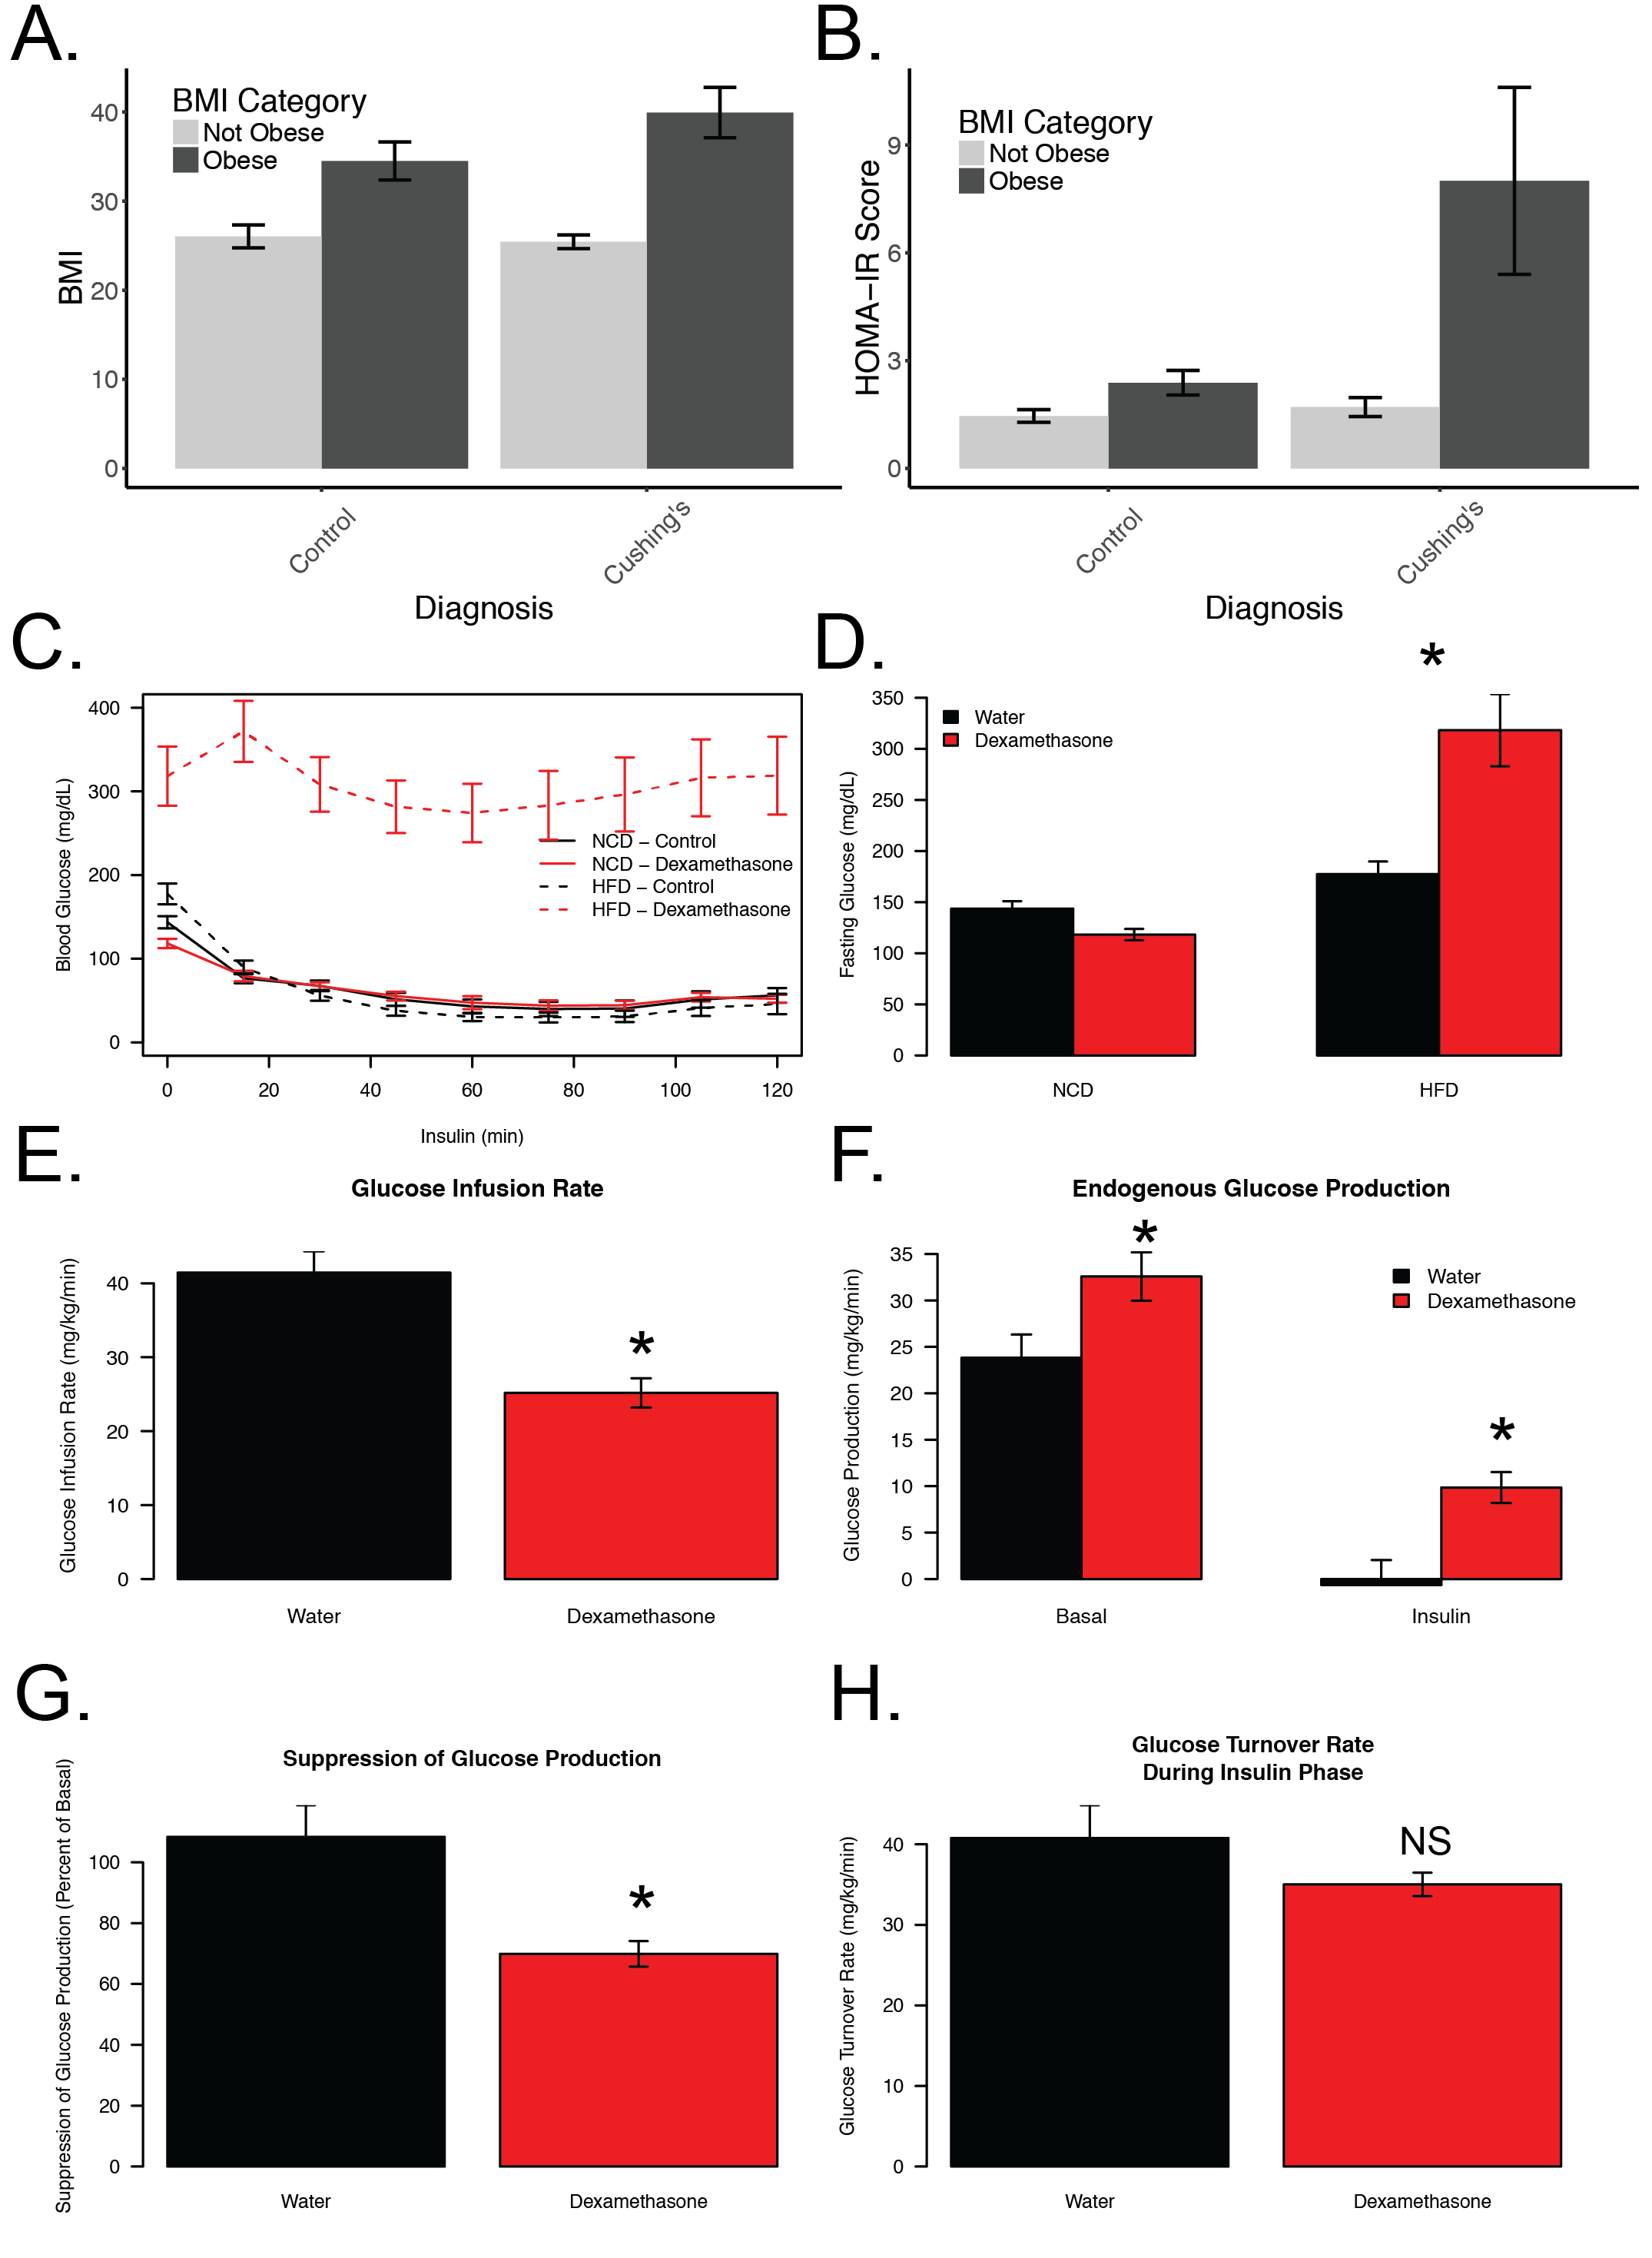
\includegraphics[width=\textwidth]{Figures_Figure_1.png}
  \end{center}
  \caption{\textbf{Reductions in glucose handling are exacerbated when
elevated glucocorticoids and obesity are combined. } Mouse blood glucose levels during insulin tolerance test (C) and prior
to insulin injection (basal; D). Insulin was given via i.p. injection at
a concentration of 2.5 U/kg following five weeks of dexamethasone (NCD
n=12; HFD n=12) or vehicle (NCD n=12; HFD n=12) treatment and 17 weeks
of diet. Mouse glucose infusion rate (GIR; E) and endogenous glucose
production (EGP; F) during euglycemic clamp following 3 weeks of
dexamethasone (n=14) or vehicle (n=11) treatment and 11 weeks of HFD.
For clamp experiments, insulin was infused at 8 mU/kg/min following a
prime continuous infusion of 40mU/kg bolus. All mice were fasted for 5-6
hours prior to experiments. Crosses indicate a significant interaction
between diet and treatment. Asterisks indicate a statistically
significant treatment effect for the pairwise comparison.}
 \label{fig:1}
\end{figure}

To evaluate glucose homeostasis in more detail we performed
hyperinsulinemic-euglycemic clamps in obese mice (11 weeks of HFD)
treated with dexamethasone for the final three weeks. This shorter
HFD/dexamethasone exposure still caused dramatic insulin resistance,
hyperglycemia and reductions in lean mass (Supplementary Figures 1A-D).
Animals were clamped while conscious and glucose levels during the clamp
as well as insulin turnover rate were similar between groups
(Supplementary Figure 1E,F). During the hyperinsulinemic phase, the
glucose infusion rate was 39\% lower in obese dexamethasone-treated mice
when compared to obese controls indicating insulin resistance at
euglycemia (Figure 1C). Basal endogenous glucose production (EGP) was
37\% higher in the dexamethasone- treated group (p=0.026). Moreover, in
the control group, EGP was reduced to near zero by a high dose of
insulin but only reduced 70\% in the dexamethasone group (p=0.0091)
resulting in glucose production being higher during the insulin phase in
dexamethasone-treated mice (p=0.014) when compared to controls (Figure
1D-E). Glucose turnover was slightly decreased in the presence of
insulin (p=0.141; Figure 1F). Despite these modest changes in glucose
turnover, there were significant reductions in the obese,
dexamethasone-treated animals in 2-deoxyglucose uptake in heart (34\%
reduced, p=0.0003) and gastrocnemius tissues (68\% reduced; p=0.00002;
Supplementary Figures 1G-H). These data suggest that increased glucose
production and its impaired suppression by insulin are the likely causes
of poor glycemic control in obese, dexamethasone-treated animals.

\subsection*{HFD-Induced Liver Steatosis in Dexamethasone-Treated
mice}

Obesity and chronic elevations in glucocorticoids are associated with
NAFLD (Wanless \& Lentz 1990; Rockall \emph{et al.} 2003). H\&E staining
of hepatic tissue clearly depicts exacerbated lipid levels in the obese,
dexamethasone-treated group when compared to obese controls and lean
groups (Figure 2A). In support of this, we observe drastically elevated
liver triglycerides when compared to all other groups with a significant
interaction between drug and diet (p=0.000068; Figure 2B).

\begin{figure}
  \begin{center}
    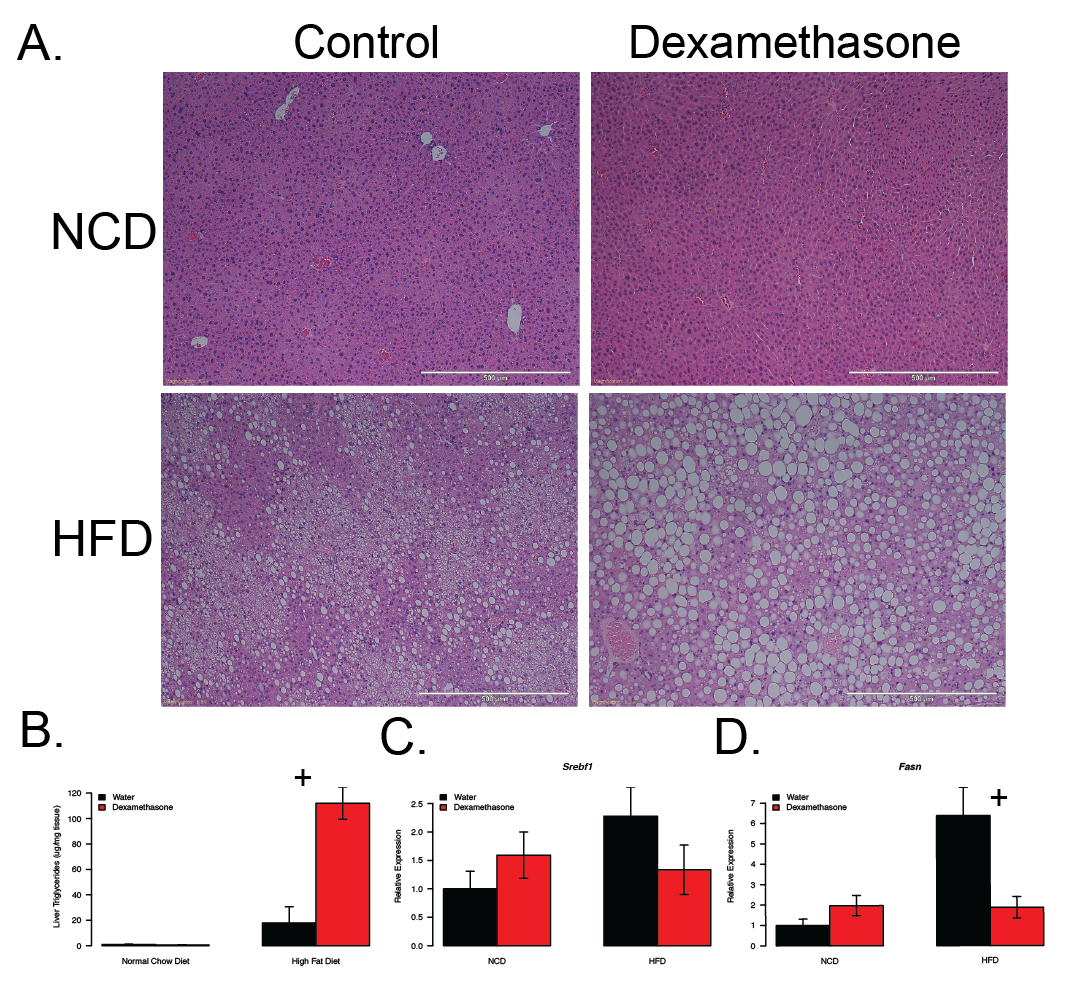
\includegraphics[width=\textwidth]{Figures_Figure_2.png}
  \end{center}
  \caption{\textbf{Increased glucocorticoids lead to greater severity of
hepatic steatosis in obese mice.}
Mouse hepatic triglyceride levels (B) and Hematoxylin and Eosin stained
liver sections (C) and qPCR of hepatic \emph{de novo} lipogenic
transcripts (D, E). Mice were euthanized at 28 weeks of age following
six weeks of dexamethasone (NCD n=7; HFD n=5) or vehicle (NCD n=6; HFD
n=9) treatment and 18 weeks of diet. Liver stains are representative
samples from each group. Crosses indicate a significant interaction
between diet and treatment.}
 \label{fig:2}
\end{figure}

We used qPCR to measure the expression of genes involved in hepatic
\emph{de novo} lipogenesis, \emph{Srebf1} and \emph{Fasn}, in liver
lysates (Figure 2C-D). We observed no synergism in expression levels
between HFD and dexamethasone. This finding indicates that lipid
accumulation in response to dexamethasone treatment is likely occurring
via mechanisms other than accelerated glucocorticoid-dependent
activation of \emph{de novo} lipogenesis.

\subsection*{Dexamethasone Causes Decreased Fat Mass in Obese
Mice}

To understand the how dexamethasone effects body composition in these
animals, we determined total fat mass. We observed reductions in fat
mass in the HFD-fed dexamethasone-treated group (Figure 3A-B). These
reductions do not appear to be depot-specific, as we observed reductions
in both iWAT (65\% reduced) and eWAT mass (59\% reduced; Figure 3C) ub
the obese, dexamethasone-treated mice. There were no significant
differences in fat mass, either by MRI or gross tissue weights of iWAT
or eWAT depots in response to dexamethasone treatment in the chow-fed
groups (Figure 3B-C). To determine if changes in body composition could
be explained by altered caloric consumption (Figure 3D), we compared
food intake among the groups. Chow-fed, dexamethasone-treated mice ate
significantly less than chow-fed controls (9\% reduction; p=0.006), as
previously reported (Haber \& Weinstein 1992; Roussel \emph{et al.}
2003). Surprisingly, we found that the dexamethasone-treated HFD-fed
animals ate slightly more food (11\% increase, p=0.032), even though
they lost both fat and fat-free mass. These data suggest that the weight
loss in obese animals provided dexamethasone is not due to reductions in
food intake.

\begin{figure}
  \begin{center}
    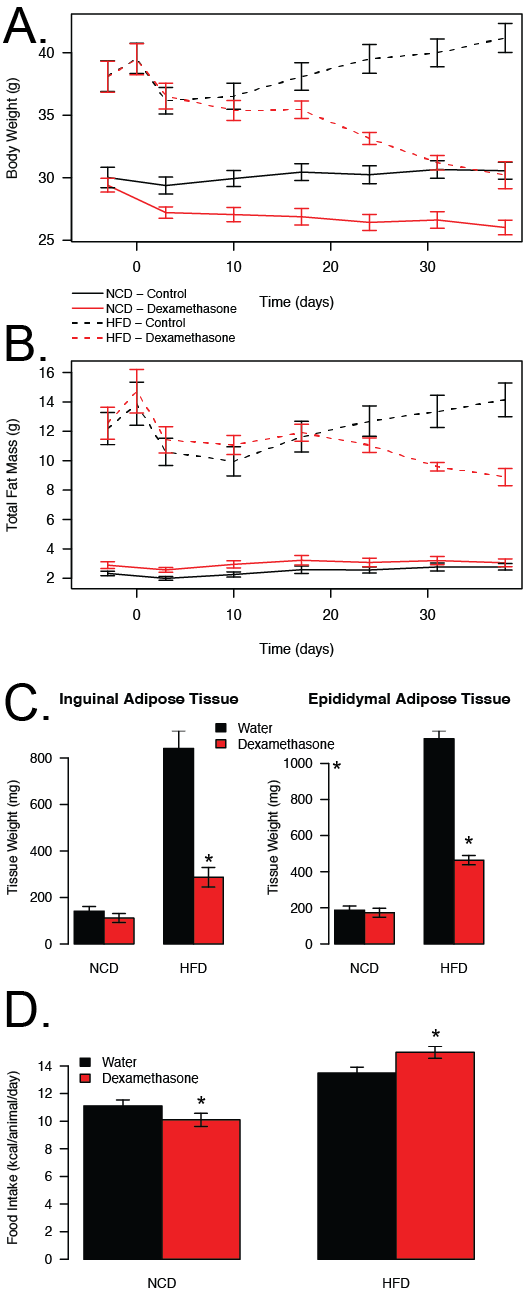
\includegraphics[width=0.5\textwidth]{Figures_Figure_3.png}
  \end{center}
  \caption{\textbf{Dexamethasone treatment reduces fat mass in obese
mice. }  Weekly total body mass (A) and fat mass (B) measures via EchoMRI in mice
over the course of treatment (solid lines represent NCD mice and dashed
lines represent HFD mice). Adipose tissue weights in 16 hour fasted mice
following euthanasia (C). Mice were euthanized at 28 weeks of age
following six weeks of dexamethasone (NCD n=8; HFD n=12) or vehicle (NCD
n=8; HFD n=22) treatment and 18 weeks of diet. Food consumption measured
weekly over the course of treatment (D). Asterisks indicate a
statistically significant treatment effect for the pairwise comparison.}
 \label{fig:3}
\end{figure}

\subsection*{Dexamethasone Treatment Results in Increased Lipolysis}

Lipolysis has previously been associated with insulin resistance (Rebrin
\emph{et al.} 1996; Edgerton \emph{et al.} 2017), is known to be
elevated in patients with NAFLD (Gastaldelli \emph{et al.} 2009), and
has been shown to increase with high levels of glucocorticoids (Djurhuus
\emph{et al.} 2002, 2004; Kršek \emph{et al.} 2006; Hochberg \emph{et
al.} 2015). To assess whether dexamethasone was affecting the lipid
content in adipose tissue, we measured markers of adipocyte lipolysis in
cultured adipocytes. 3T3-L1 fibroblasts were undifferentiated
(pre-adipocytes); or differentiated and treated with vehicle or
dexamethasone following differentiation. Dexamethasone treatment
following differentiation led to decreased lipid content (52.4\%
reduction, p=0.005) and a 71\% increase in the amount of glycerol in the
media (p=0.001), suggesting increased lipolysis (Figure 4B). In order to
identify a potential GR-dependent lipolytic target, we evaluated the
levels of ATGL, the rate limiting enzyme in lipolysis. Expression of
ATGL (encoded by the \emph{Pnpla2} gene) was enhanced following
dexamethasone treatment in 3T3-L1 cells at the transcript (2.7 fold,
p=0.002; Figure 4C) and protein (4.2 fold, p=0.025; Figure 4D-E) levels.
These data show that glucocorticoids elevate ATGL levels and metabolites
of lipolysis in cultured adipocytes.

\begin{figure}
  \begin{center}
    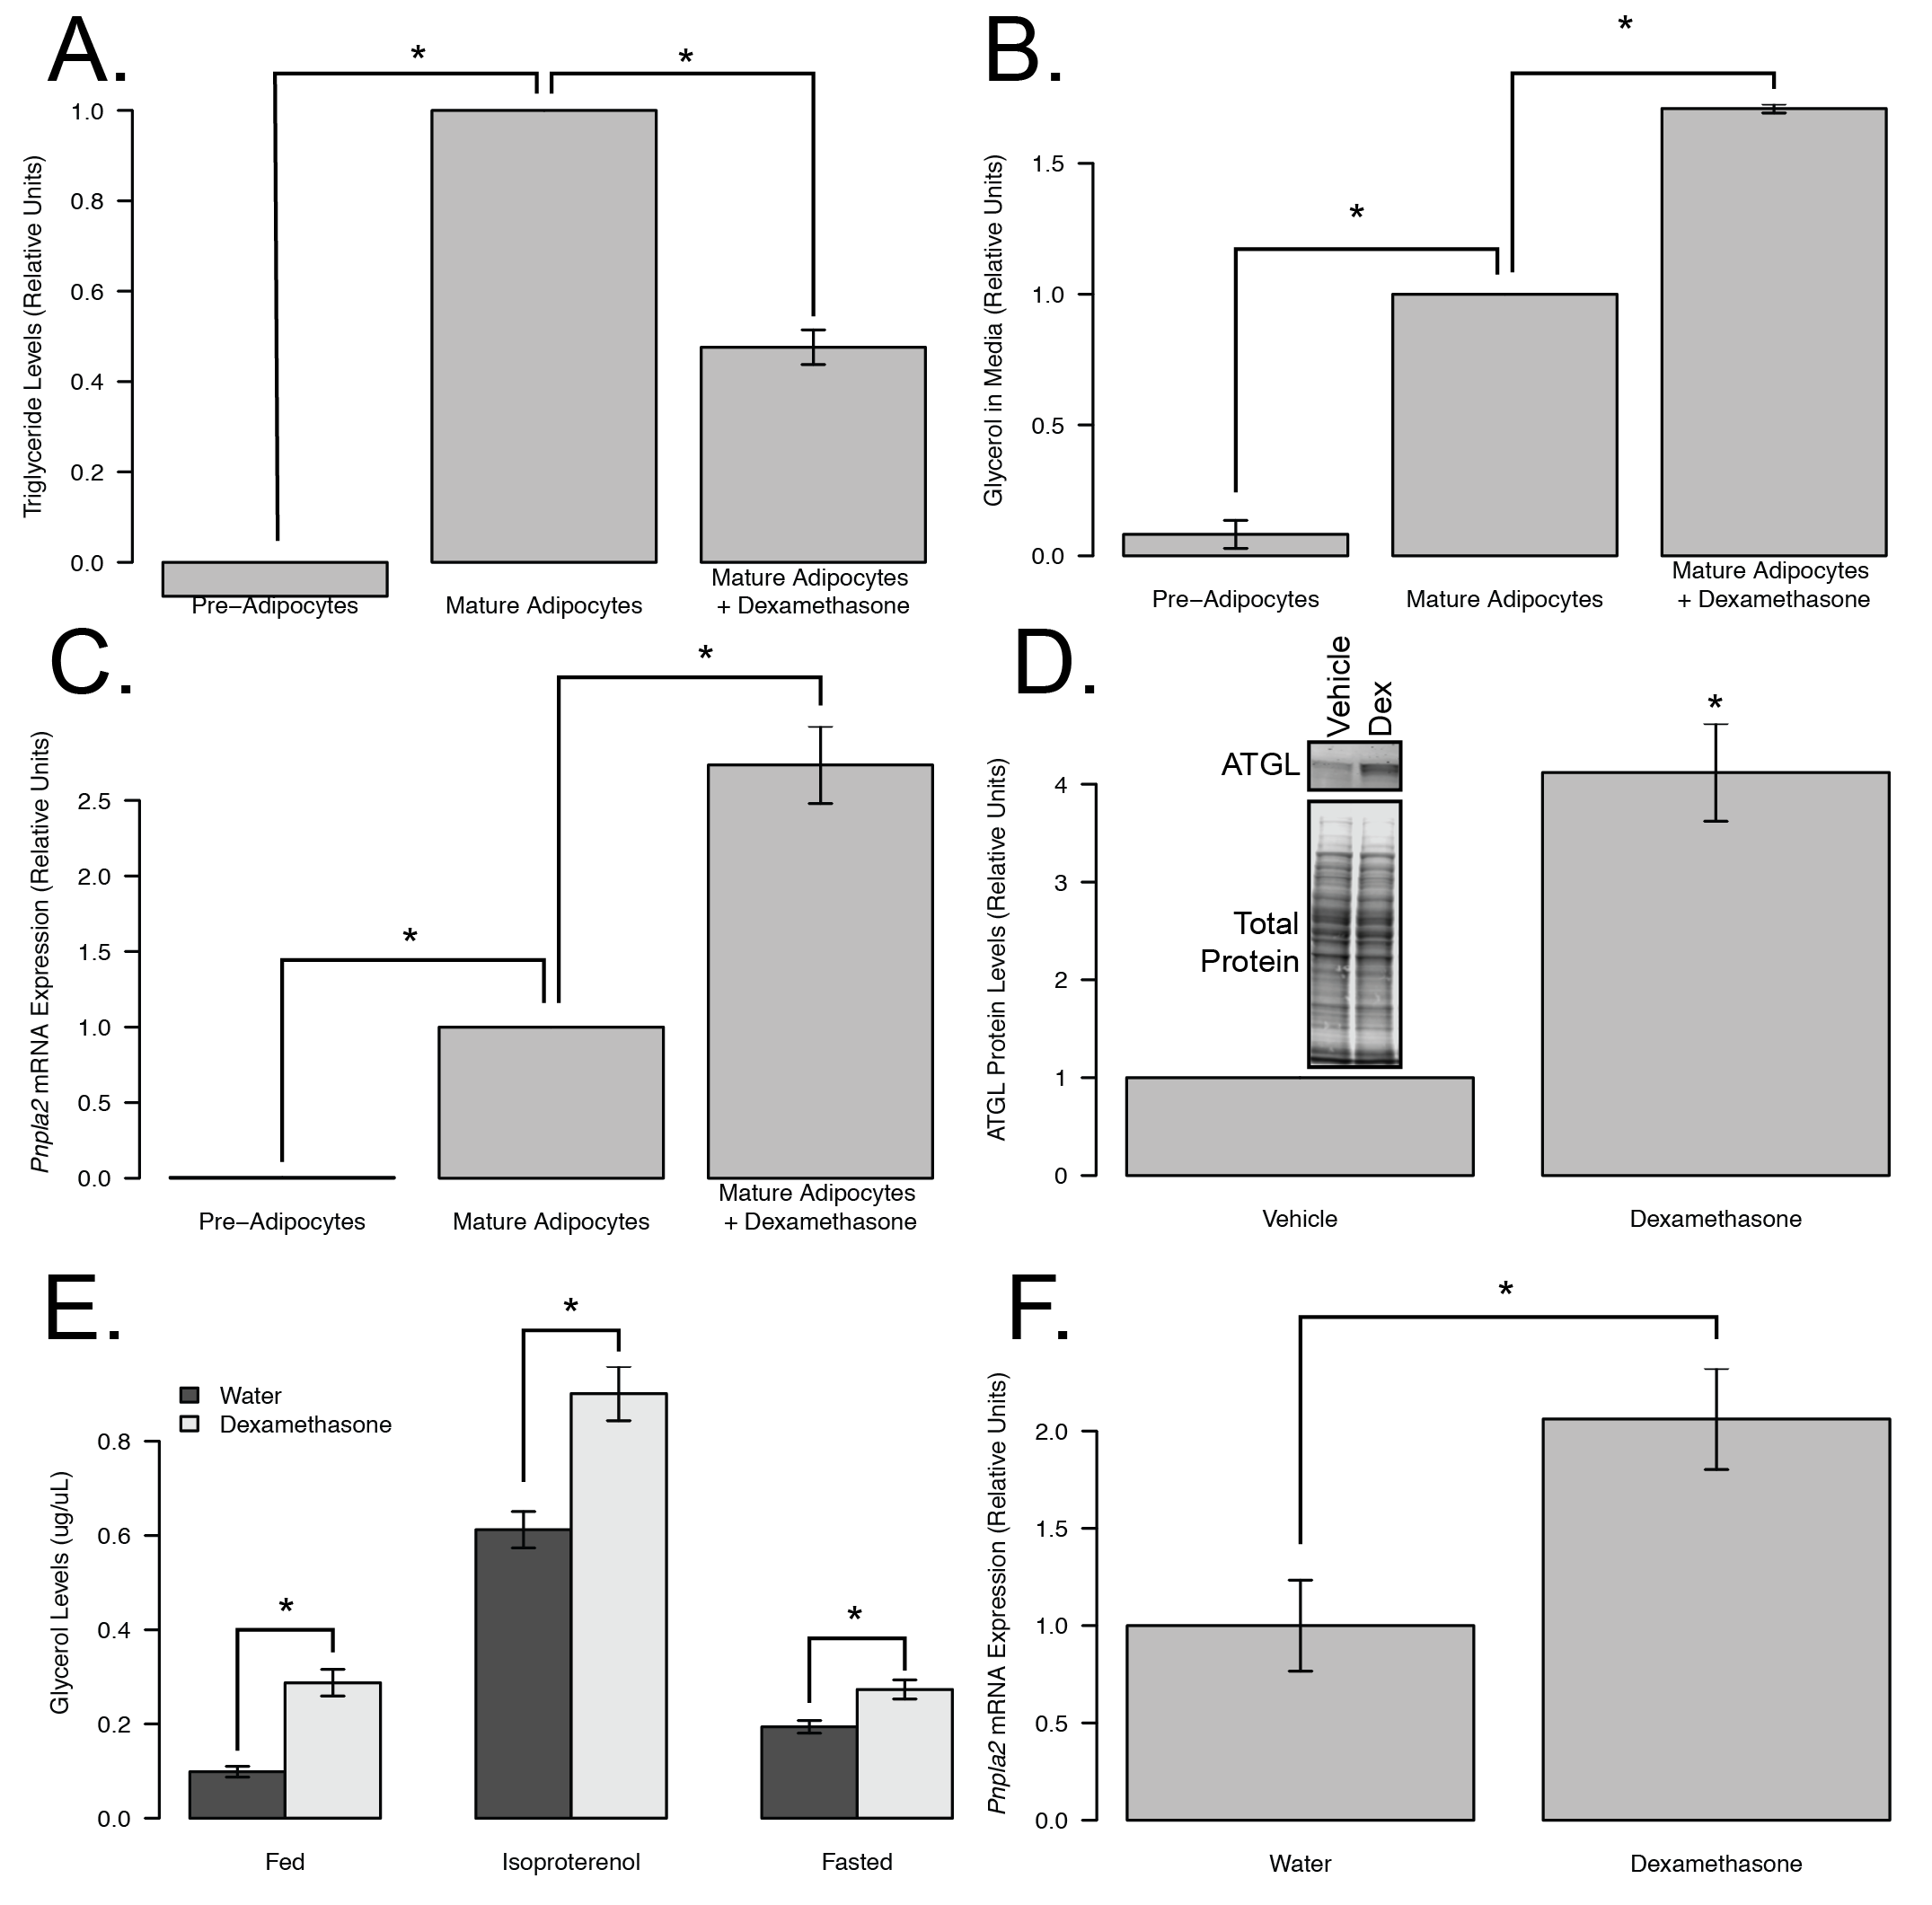
\includegraphics[width=0.4\textwidth]{Figures_Figure_4.png}
  \end{center}
  \caption{
\textbf{Dexamethasone treatment induces lipolysis \emph{in
vivo} and \emph{in vitro}.}  Triglyceride levels (A), glycerol released in media (B), qPCR of
lipolytic transcripts (C), and western blot of ATGL (D) from
non-differentiated (pre-adipocytes; n=2) or differentiated 3T3-L1 mouse
adipocytes (mature adipocytes) following five days of dexamethasone
(n=3) or vehicle treatment (n=3). Serum fatty acid and glycerol levels
at basal (fed) and following stimulation (10mg/kg isoproterenol or 16hr
fast; E) and qPCR of IWAT lipolytic transcripts (F) in 22-week-old,
12-week dexamethasone- (basal and isoproterenol n=7; fasted serum and
qPCR n=4) or vehicle- (basal and isoproterenol n=12; fasted serum and
qPCR n=11) treated, chow-fed mice with the exception of
isoproterenol-stimulated glycerol, which was performed one week prior to
euthanasia. Asterisks indicated statistically significant treatment
effect for the pairwise comparison.}
 \label{fig:4}
\end{figure}

To measure the effects of glucocorticoid-induced lipolysis \emph{in
vivo,} we quantified glycerol levels in animals chronically exposed to
dexamethasone in basal and stimulated conditions (Figure 4E).
Stimulation of lipolysis was achieved via isoproterenol, a $\beta$-adrenergic
receptor agonist, or by a 16-hour fast. Dexamethasone treatment led to
increases in glycerol in the fed (2.9 fold), fasted (1.5 fold) and
isoproterenol-stimulated (1.4 fold) conditions (p\textless{}0.05 for all
pairwise comparisons), indicating that dexamethasone enhances basal and
stimulated lipolysis \emph{in vivo} in chow-fed mice. Consistent with
these findings, mRNA analysis from iWAT of these mice showed an
upregulation of \emph{Pnpla2} transcripts in the dexamethasone-treated
mice compared to controls (2.1 fold, p=0.016; Figure 4F).

To understand how diet-induced obesity alters dexamethasone-induced
lipolysis, we next quantified serum glycerol concentrations in our
HFD/NCD fed mice (Figure 5A). We observed a nearly two-fold increase in
serum glycerol levels by dexamethasone treatment in the HFD-fed animals,
compared with only a 18\% increase in chow-fed mice (p=0.017 for the
interaction between diet and dexamethasone). For the hyperinsulinemic
euglycemic clamp in the obese mice there was a 40\% elevation in serum
basal non-esterified fatty acids (NEFA's) in response to 3 weeks of
dexamethasone treatment (p=0.004; Figure 5B). During the insulin phase,
dexamethasone treatment attenuated the ability of insulin to suppress
serum NEFA levels with insulin leading to a 71\% reduction in controls
compared to only a 48\% reduction in dexamethasone-treated mice
(p=0.058). These findings suggest that in the obese setting,
dexamethasone elevates lipolysis to a greater extent and attenuates the
effects of insulin.

\begin{figure}
  \begin{center}
    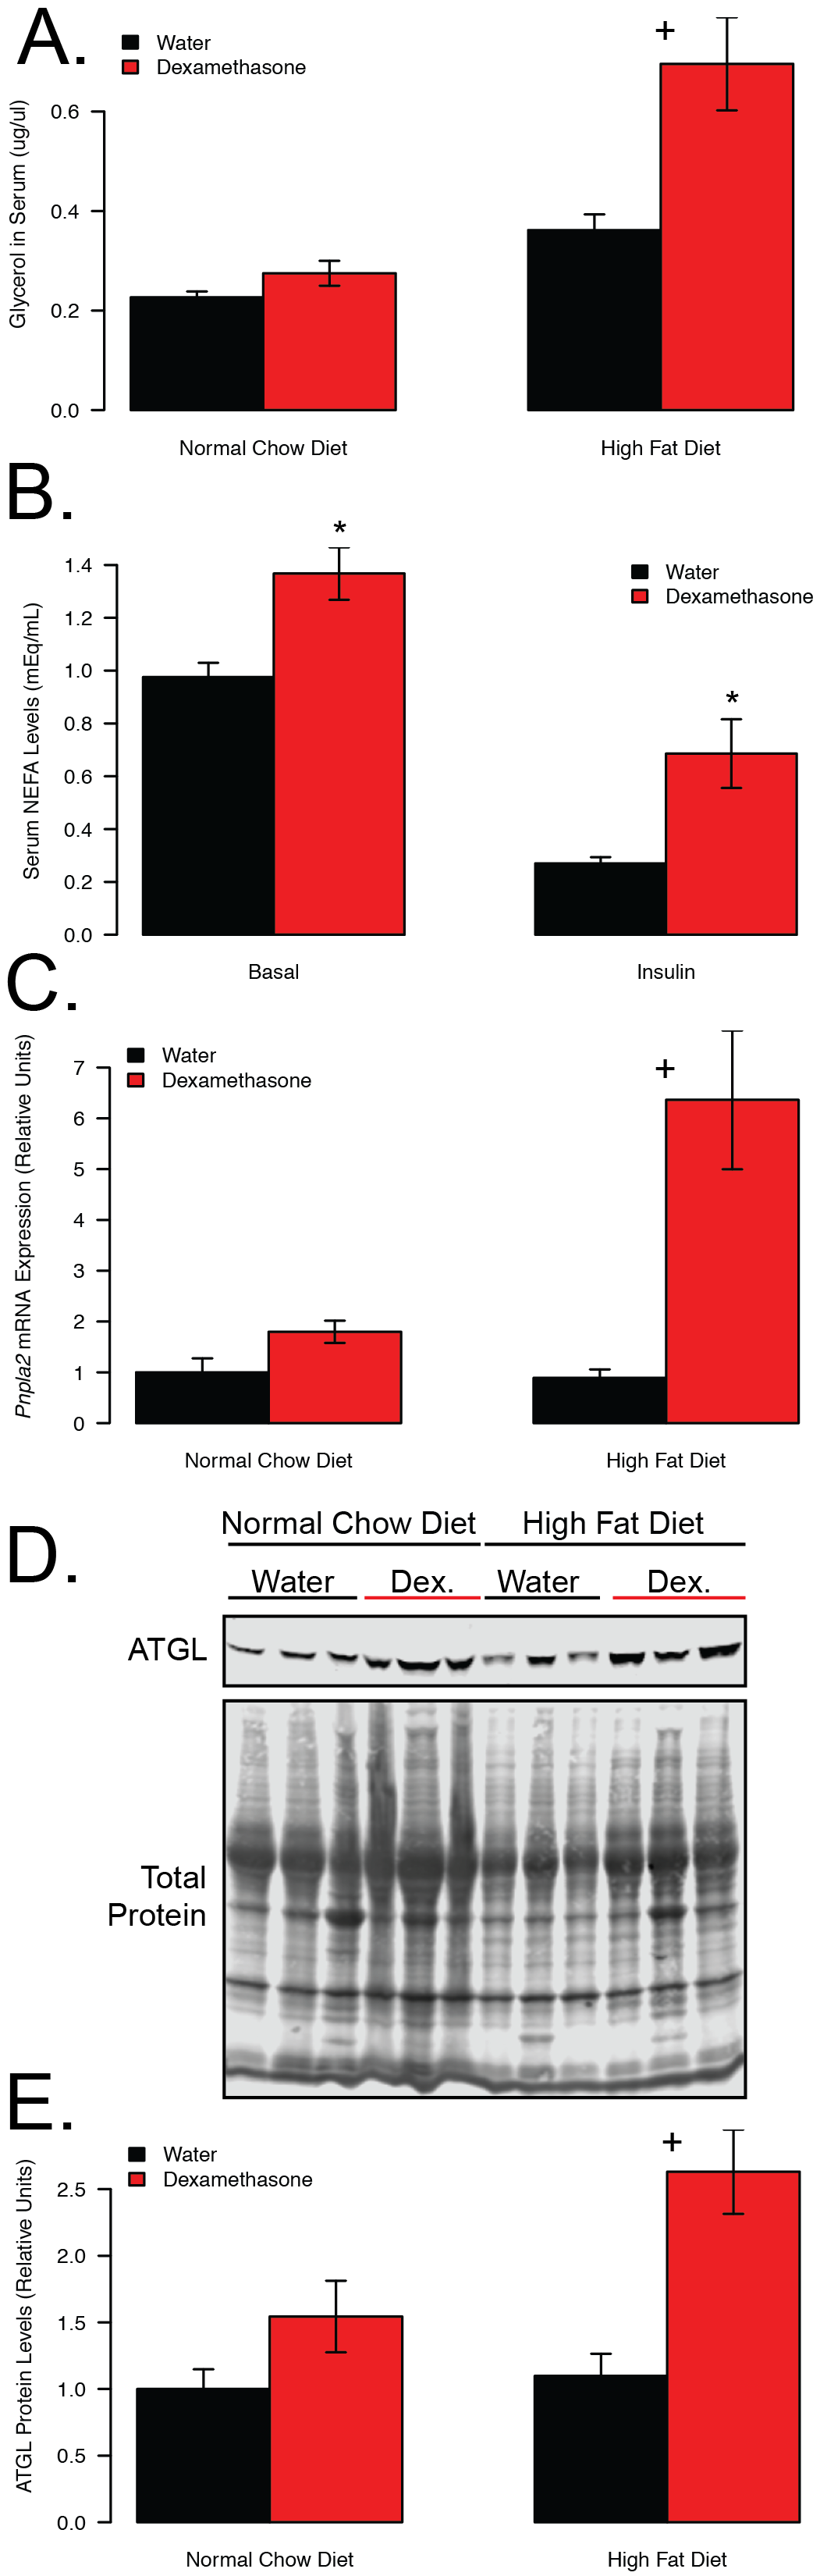
\includegraphics[width=0.4\textwidth]{Figures_Figure_5.png}
  \end{center}
  \caption{\textbf{Obesity exacerbates dexamethasone-induced lipolysis. }
Serum glycerol (A) following 16 hour fast, serum NEFA in obese
dexamethasone treated (n=14) or control (n=11) mice following a 5 hour
fast, before and after insulin during hyperinsulinemic euglycemic clamp
(B), qPCR of \emph{Pnpla2} transcripts from iWAT (C), and western blot
image (D) and quantification (E) of ATGL protein from iWAT. Mice from A,
C, D and E were euthanized at 28 weeks of age following six weeks of
dexamethasone (NCD n=8; HFD n=10) or vehicle (NCD n=8; HFD n=10)
treatment. Crosses indicate a significant interaction between diet and
treatment. Asterisks indicate a statistically significant treatment
effect for the pairwise comparison.}
 \label{fig:5}
\end{figure}

To investigate the molecular basis for this synergistic increase in
lipolysis, we quantified mRNA and protein expression of ATGL in the iWAT
of these mice (5C-E). Consistent with the hypothesis that ATGL
activation could drive increased lipolysis in obese
dexamethasone-treated mice, expression of ATGL was elevated in both
dexamethasone-treated groups, with a significant synergistic effect of
dexamethasone and obesity at the transcript (p=0.02) and protein
(p=0.043) levels. These data support the hypothesis that
glucocorticoid-stimulated lipolysis is augmented in the context of
obesity, potentially via increased transactivation of
\emph{Pnpla2}/ATGL.

\section*{Discussion}

Chronic glucocorticoid elevations are associated with co-morbidities
such as increased fat mass (Abad \emph{et al.} 2001; Geer \emph{et al.}
2011; Hochberg \emph{et al.} 2015), decreased muscle mass (Dardevet
\emph{et al.} 1995; Schakman \emph{et al.} 2013; Hochberg \emph{et al.}
2015), insulin resistance and NAFLD (Paredes \& Ribeiro 2014). Many of
these adverse effects are similar to those seen in obesity; however, the
combination of chronically elevated glucocorticoids in the context of
pre-existing obesity has not been assessed. Here, we show that the
effects of glucocorticoid-induced insulin resistance and NAFLD are
exacerbated when paired with obesity.

We appreciate that glucocorticoids directly affect many other tissues,
such as muscle, liver and the pancreas that may also influence insulin
sensitivity. In support of a central role of adipocytes, several studies
demonstrate that adipocyte-specific reductions in glucocorticoid
signaling being associated with improved metabolic profiles (Morgan
\emph{et al.} 2014; Wang \emph{et al.} 2014; Mueller \emph{et al.} 2017;
Shen \emph{et al.} 2017). We hypothesize that adipose tissue lipolysis
plays a major role in dexamethasone-induced insulin resistance and
hepatic steatosis, especially in the case of obesity.

Excess adiposity, such is seen in obesity, has been associated with
increased insulin resistance. Previous work from our lab shows increased
fat mass following 12 weeks of dexamethasone treatment (Hochberg
\emph{et al.} 2015) in lean mice, in accordance with what others have
reported (Burke \emph{et al.} 2017), as well as reduced insulin
sensitivity. However, to our surprise, the glucocorticoid treatment in
obese mice led to a lipodystrophic phenotype, which indicates the
disturbances in glucose homeostasis are not a result of increased fat
mass. The loss in fat mass observed in the obese, dexamethasone treated
mice was not due to reduced food intake, in fact these mice ate
significantly more calories per day than obese controls. This suggests a
potential increase in energy expenditure with the combination of obesity
and dexamethasone treatment over time. This study evaluated
glucocorticoid treatment in the context of diet-induced obesity;
however, Riddell and colleagues have reported similar findings when
providing HFD and glucocorticoids in concert to rats, prior to the onset
of obesity (D'souza \emph{et al.} 2012; Shpilberg \emph{et al.} 2012;
Beaudry \emph{et al.} 2013). It is not clear whether diet or obesity
status have similar mechanisms causing exacerbated metabolic risk, but
these interactions deserve further evaluation.

Lipolysis has been linked to increased gluconeogenesis by several
studies (Williamson \emph{et al.} 1966; Nurjhan \emph{et al.} 1986,
1992, Perry \emph{et al.} 2015, 2017). Glucocorticoids are known to
stimulate lipolysis (Djurhuus \emph{et al.} 2002, 2004; Kršek \emph{et
al.} 2006; Hochberg \emph{et al.} 2015), possibly as a way to promote
gluconeogenesis to maintain blood glucose levels. Lipolysis has been
implicated in insulin resistance (Rebrin \emph{et al.} 1996; Edgerton
\emph{et al.} 2017) and NAFLD (Gastaldelli \emph{et al.} 2009). We found
synergistic elevations in glycerol, indicative of enhanced lipolysis, as
well as in hepatic fat accumulation in the HFD-fed,
dexamethasone-treated mice, but no data supporting enhanced hepatic
\emph{de novo} lipogenesis. Therefore, we propose the
dexamethasone-induced increase in hepatic steatosis in the obese mice is
primarily due to enhanced lipolysis observed in these animals.

There is some debate as to which genes glucocorticoids are acting on to
promote lipolysis. Downregulation of \emph{Pde3b} (Xu \emph{et al.}
2009) and upregulation of $\beta$-adrenergic receptors (Lacasa \emph{et al.}
1988) and ATGL transcripts (Campbell \emph{et al.} 2011; Serr \emph{et
al.} 2011; Shen \emph{et al.} 2017) have been proposed as possible
mechanisms. We found ATGL, the rate limiting enzyme for adipose
triglyceride lipolysis, to be synergistically activated by obesity and
glucocorticoid-treatment. These findings bear a resemblance to
elevations in glycerol levels in obese, dexamethasone-treated mice when
compared to diet or glucocorticoids alone. The mechanisms by which
obesity and glucocorticoids synergize to activate ATGL expression are
not clear at this time, nor are the relative contributions of other
glucocorticoid receptor-dependent targets.

In summary, glucocorticoids are commonly prescribed drugs used to treat
a multitude of health issues, but are known to induce a variety of
adverse metabolic effects. Their actions in persons with obesity are not
yet clear, even though there is a significant number of individuals with
obesity routinely taking prescription glucocorticoids. This paper is the
first to show that diet-induced obesity in mice exacerbates several
co-morbidities associated with chronically elevated glucocorticoids.
These effects may be considered by physicians when determining
glucocorticoid treatment options for patients with obesity.

\textbf{Declaration of Interest:} The authors declared no conflict of
interest that could be perceived as prejudicing the impartiality of the
research reported.

\textbf{Funding:} This study was supported by funds from NIH Grant
R01-DK107535 (DB) and a~Pilot and Feasibility Grant from the Michigan
Diabetes Research Center (P30-DK020572). This study also utilized the
University of Michigan Metabolism, Bariatric Surgery and Behavior Core
(U2C-DK110768), the Michigan Nutrition Obesity Research Center
(P30-DK089503) and the University of Michigan Comprehensive Cancer
Center Core (P30-CA062203). Erin Stephenson is partially supported by
funding from Le Bonheur Children's Hospital, the Children's Foundation
Research Institute and the Le Bonheur Associate Board.

\textbf{Author contributions:} D.B. acquired funding. D.B., I.Ha. and
I.Ho. were responsible for conceptualizing the study. D.B., I.Ha. and
N.Q. designed the experiments. I.Ha. performed all cell experiments.
I.Ha., E.S. and J.R. performed mouse experiments. D.B. and Q.T.
performed statistical analyses. I.Ha. wrote the manuscript. I.Ha. and
D.B. edited and reviewed the manuscript. All authors were involved in
discussions. This manuscript has been approved by all authors.

\textbf{Acknowledgements:} We would like to thank the study participant
for their willingness to be involved in this research. We would like to
thank Jennifer DelProposto and Carey Lumeng for assistance with imaging
liver sections, and Melanie Schmitt for assistance with glucose clamp
studies. We would like to thank the other members of the Bridges
laboratory, Thurl Harris (University of Virginia), Christoph Buettner
and Eliza Geer (Icahn School of Medicine at Mount Sinai) and Edwards
Park (UTHSC) for insights on this work. g

\section*{References}

Abad V, Chrousos GP, Reynolds JC, Nieman LK, Hill SC, Weinstein RS \&
Leong GM 2001 Glucocorticoid Excess During Adolescence Leads to a Major
Persistent Deficit in Bone Mass and an Increase in Central Body Fat.
\textbf{16} 1879--1885.

Ayala JE, Bracy DP, Mcguinness OP \& Wasserman DH 2006 Considerations in
the Design of Hyperinsulinemic- Euglycemic Clamps in the Conscious
Mouse.

Beaudry JL, Anna MD, Teich T, Tsushima R \& Riddell MC 2013 Exogenous
Glucocorticoids and a High-Fat Diet Cause Severe Hyperglycemia and
Hyperinsulinemia and Sprague-Dawley Rats. \textbf{154} 3197--3208.
(doi:10.1210/en.2012-2114)

Burke SJ, Batdorf HM, Eder AE, Karlstad MD, Burk DH, Noland RC, Floyd ZE
\& Collier JJ 2017 Oral Corticosterone Administration Reduces Insulitis
but Promotes Insulin Resistance and Hyperglycemia in Male Nonobese
Diabetic Mice. \emph{The American Journal of Pathology} \textbf{187}
614--626. (doi:10.1016/j.ajpath.2016.11.009)

Campbell JE, Peckett AJ, D'souza AM, Hawke TJ \& Riddell MC 2011
Adipogenic and lipolytic effects of chronic glucocorticoid exposure.
\emph{American Journal of Physiology. Cell Physiology} \textbf{300}
C198-209. (doi:10.1152/ajpcell.00045.2010)

Chiang S-H, Chang L SA 2002 TC10 and Insulin ‐ Stimulated Glucose
Transport. \textbf{406} 1257--1262. (doi:10.1016/S0076-6879(06)06055-1)

D'souza AM, Beaudry JL, Szigiato AA, Trumble SJ, Snook LA, Bonen A,
Giacca A \& Riddell MC 2012 Consumption of a high-fat diet rapidly
exacerbates the development of fatty liver disease that occurs with
chronically elevated glucocorticoids. \emph{American Journal of
Physiology Gastrointestinal Liver Physiology} \textbf{302} 850--863.
(doi:10.1152/ajpgi.00378.2011)

Dardevet D, Somet C, Taillandier D, Savary I, Attaix D \& Grizard J 1995
Sensitivity and Protein Turnover Response to Glucocorticoids Are
Different in Skeletal Muscle from Adult and Old Rats Lack of Regulation
of the Ubiquitin-Proteasome Proteolytic Pathway in Aging. \emph{Journal
of Clinical Investigation} \textbf{96} 2113--2119.

Dirks ML, Wall BT, Valk B Van De \& Holloway TM 2016 One Week of Bed
Rest Leads to Substantial Muscle Atrophy and Induces Whole-Body Insulin
Resistance in the Absence of Skeletal Muscle Lipid Accumulation.
\textbf{65} 2862--2875. (doi:10.2337/db15-1661)

Djurhuus CB, Gravholt CH, Nielsen S, Mengel a, Christiansen JS, Schmitz
OE \& Møller N 2002 Effects of cortisol on lipolysis and regional
interstitial glycerol levels in humans. \emph{American Journal of
Physiology. Endocrinology and Metabolism} \textbf{283} E172--E177.
(doi:10.1152/ajpendo.00544.2001)

Djurhuus CB, Gravholt CH, Nielsen S, Pedersen SB, Møller N \& Schmitz O
2004 Additive effects of cortisol and growth hormone on regional and
systemic lipolysis in humans. 488--494.

Edgerton DS, Kraft G, Smith M, Farmer B, Williams PE, Coate KC, Printz
RL, Brien RMO \& Cherrington AD 2017 Insulin ' s direct hepatic effect
explains the inhibition of glucose production caused by insulin
secretion. \textbf{2} 1--14.

Fardet L, Petersen I \& Nazareth I 2011 Original article Prevalence of
long-term oral glucocorticoid prescriptions in the UK over the past 20
years. (doi:10.1093/rheumatology/ker017)

Gastaldelli A, Harrison SA, Belfort-aguilar R, Hardies LJ, Balas B,
Schenker S \& Cusi K 2009 Importance of Changes in Adipose Tissue
Insulin Resistance to Histological Response During Thiazolidinedione
Treatment of Patients with Nonalcoholic Steatohepatitis.
(doi:10.1002/hep.23116)

Geer EB, Shen W, Gallagher D, Punyanitya M, Looker HC, Post KD \& Freda
PU 2011 Female Patients with Cushing ' s Disease. \textbf{73} 469--475.
(doi:10.1111/j.1365-2265.2010.03829.x.MRI)

Haber RS \& Weinstein SP 1992 Role of Glucose Transporters in
Glucocorticoid-lnduced Insulin Resistance GLUT4 Isoform in Rat Skeletal
Muscle is Not Decreased by Dexamethasone. \textbf{41} 728--735.

Halseth AMYE, Bracy DP, Wasserman DH, Amy E, Bracy DP \& David H 1999
Overexpression of hexokinase II increases insulin- and
exercise-stimulated muscle glucose uptake in vivo.

Hochberg I, Harvey I, Tran QT, Stephenson EJ, Barkan AL, Saltiel AR,
Chandler WF \& Bridges D 2015 Gene expression changes in subcutaneous
adipose tissue due to Cushing's disease. \emph{Journal of Molecular
Endocrinology} \textbf{55} 81--94. (doi:10.1530/JME-15-0119)

Hsiao C, Ph D, Cherry DK, Beatty PC, Ph D, Rechtsteiner EA \& Care H
2010 National Ambulatory Medical Care Survey : 2007 Summary.

Kraegen E, James D, Jenkins A \& Chisholm D 1985 Dose-response curves
for in vivo insulin sensitivity in individual tissues in rats. \emph{The
American Physiological Society} E353--E362.

Kršek M, Rosická M, Nedvídková J, Ková HKČ, Hána V, Marek J, Haluzík M,
Lai EW \& Pacák K 2006 Increased Lipolysis of Subcutaneous Abdominal
Adipose Tissue and Altered Noradrenergic Activity in Patients with
Cushing ` s Syndrome : An In-vivo Microdialysis Study. 421--428.

Lacasa D, Agli B \& Giudicelli Y 1988 PERMISSIVE ACTION OF
GLUCOCORTICOIDS ON CATECHOLAMINE-INDUCED LIPOLYSIS : DIRECT `IN VITRO'
EFFECTS ON THE FAT CELL
\textasciitilde{}-ADRENORECEPTOR-COUPLED-ADENYLATE CYCLASE SYSTEM
Dani\textasciitilde{}le. \emph{Biochemical and Biophysical Research
Communications} \textbf{153} 489--497.

Laugesen K, Otto J, Jørgensen L, Sørensen HT \& Petersen I 2017 Systemic
glucocorticoid use in Denmark : a population-based prevalence study.
1--6. (doi:10.1136/bmjopen-2016-015237)

Lu B, Bridges D, Yang Y, Fisher K, Cheng A, Chang L, Meng ZX, Lin JD,
Downes M, Yu RT \emph{et al.} 2014 Metabolic crosstalk: Molecular links
between glycogen and lipid metabolism in obesity. \emph{Diabetes}
\textbf{63} 2935--2948. (doi:10.2337/db13-1531)

McGuinness OP, Ayala JE, Laughlin MR \& Wasserman DH 2009 NIH experiment
in centralized mouse phenotyping: the Vanderbilt experience and
recommendations for evaluating glucose homeostasis in the mouse.
\emph{American Journal of Physiology - Endocrinology and Metabolism}
\textbf{297}.

Morgan SA, McCabe EL, Gathercole LL, Hassan-Smith ZK, Larner DP,
Bujalska IJ, Stewart PM, Tomlinson JW \& Lavery GG 2014 11$\beta$-HSD1 is the
major regulator of the tissue-specific effects of circulating
glucocorticoid excess. \emph{Proceedings of the National Academy of
Sciences of the United States of America}. (doi:10.1073/pnas.1323681111)

Mueller KM, Hartmann K, Kaltenecker D, Vettorazzi S, Bauer M, Mauser L,
Amann S, Jall S, Fischer K, Esterbauer H \emph{et al.} 2017 Adipocyte
Glucocorticoid Receptor De fi ciency Attenuates Aging- and HFD-Induced
Obesity and Impairs the Feeding-Fasting Transition. \textbf{66}
272--286. (doi:10.2337/db16-0381)

Nurjhan N, Campbell PJ, Kennedy FP, Miles JM \& Gerich JE 1986 Insulin
Dose-Response Characteristics for Suppression of Glycerol Release and
Conversion to Glucose in Humans. \textbf{35} 1326--1331.

Nurjhan N, Consoli A \& Gerich J 1992 Increased Lipolysis and Its
Consequences on Gluconeogenesis in Non-insulin-dependent Diabetes
Mellitus. \textbf{89} 169--175.

Overman R a., Yeh JY \& Deal CL 2013 Prevalence of oral glucocorticoid
usage in the United States: A general population perspective.
\emph{Arthritis Care and Research} \textbf{65} 294--298.
(doi:10.1002/acr.21796)

Paredes S \& Ribeiro L 2014 Cortisol: the villain in Metabolic Syndrome?
\emph{Rev Assoc Med BRAs} \textbf{60} 84--92.
(doi:10.1590/1806-9282.60.01.017)

Perry RJ, Camporez JG, Kursawe R, Titchenell PM, Zhang D, Perry CJ,
Jurczak MJ, Abudukadier A, Han S, Zhang X \emph{et al.} 2015 Hepatic
Acetyl CoA Links Adipose Tissue Inflammation to Hepatic Insulin
Resistance and Type 2 Diabetes. \emph{Cell} \textbf{160} 745--758.
(doi:10.1016/j.cell.2015.01.012.Hepatic)

Perry RJ, Peng L, Abulizi A, Kennedy L, Cline GW \& Shulman GI 2017
Mechanism for leptin ' s acute insulin-independent effect to reverse
diabetic ketoacidosis. \textbf{127} 657--669.

Rebrin K, Steil GM, Mittelman SD \& Bergman RN 1996 Causal Linkage
between Insulin Suppression of Lipolysis and Suppression of Liver
Glucose Output in Dogs. \textbf{98} 741--749.

Rockall A, Sohaib S, Evans D, Kaltsas G, Isidori A, Monson J, Besser G,
Grossman A \& Reznek R 2003 Hepatic steatosis in Cushing's syndrome: a
radiological assessment using computed tomography. \emph{European
Journal of Endocrinology} \textbf{149} 543--548.
(doi:10.1530/eje.0.1490543)

Roussel D, Dumas JF, Augeraud A, Douay O, Foussard F, Malthiéry Y,
Simard G \& Ritz P 2003 Dexamethasone treatment specifically increases
the basal proton conductance of rat liver mitochondria. \emph{FEBS
Letters} \textbf{541} 75--79. (doi:10.1016/S0014-5793(03)00307-7)

Schakman O, Kalista S, Barbé C, Loumaye A \& Thissen JP 2013
Glucocorticoid-induced skeletal muscle atrophy ଝ. \emph{International
Journal of Biochemistry and Cell Biology} \textbf{45} 2163--2172.
(doi:10.1016/j.biocel.2013.05.036)

Serr J, Suh Y \& Lee K 2011 Acute Up-Regulation of Adipose Triglyceride
Lipase and Release of Non-Esterified Fatty Acids by Dexamethasone in
Chicken Adipose Tissue. 813--820. (doi:10.1007/s11745-011-3583-8)

Shen Y, Roh HC, Kumari M \& Rosen ED 2017 Adipocyte glucocorticoid
receptor is important in lipolysis and insulin resistance due to
exogenous steroids , but not insulin resistance caused by high fat
feeding. \emph{Molecular Metabolism}. (doi:10.1016/j.molmet.2017.06.013)

Shpilberg Y, Beaudry JL, Souza AD, Campbell JE, Peckett A \& Riddell MC
2012 A rodent model of rapid-onset diabetes induced by glucocorticoids
and high-fat feeding. \textbf{680} 671--680. (doi:10.1242/dmm.008912)

The GBD 2015 Obesity Collaborators 2017 Health Effects of Overweight and
Obesity in 195 Countries over 25 Years. \emph{New England Journal of
Medicine} \textbf{377} 13--27. (doi:10.1056/NEJMoa1614362)

Wang Y, Yan C, Liu L, Wang W, Du H, Fan W, Lutfy K, Jiang M, Friedman TC
\& Liu Y 2014 11~-Hydroxysteroid dehydrogenase type 1 shRNA ameliorates
glucocorticoid-induced insulin resistance and lipolysis in mouse
abdominal adipose tissue. \emph{AJP: Endocrinology and Metabolism}
\textbf{308} E84--E95. (doi:10.1152/ajpendo.00205.2014)

Wanless I \& Lentz J 1990 Fatty Liver Hepatitis ( Steatohepatitis ) and
Obesity : An Autopsy Study with Analysis of Risk Factors.
\emph{Hepatology} \textbf{12} 1106--1110.

Williamson JR, Kreisberg RA \& Felts PW 1966 Mechanism for the
stimulation of gluconeogenesis by fatty acids in perfused rat liver.
\emph{Proceedings of the National Academy of Sciences of the United
States of America} \textbf{56} 247--254. (doi:10.1073/pnas.56.1.247)

Xu C, He J, Jiang H, Zu L, Zhai W, Pu S \& Xu G 2009 Direct effect of
glucocorticoids on lipolysis in adipocytes. \emph{Molecular
Endocrinology (Baltimore, Md.)} \textbf{23} 1161--1170.
(doi:10.1210/me.2008-0464)

Zhang M, Hu T, Zhang S \& Zhou L 2015 Associations of Different Adipose
Tissue Depots with Insulin Resistance : A Systematic Review and
Meta-analysis of Observational Studies. \emph{Nature Publishing Group}
1--6. (doi:10.1038/srep18495)

\end{document}
